\documentclass[a4paper,11pt,titlepage]{article}
\usepackage{graphicx}
\author{Abrie Greeff\\B.Sc Hons (Computer Science)\\Department of Computer Science\\University of Stellenbosch\\Supervisor:\\Dr. L van Zijl}

\title{Hand Motion Detection From Video Data}

\begin{document}
\maketitle

\tableofcontents
\newpage
\listoffigures
\newpage

%
% INTRODUCTION
%

\section{Introduction}
As of writing a South African Sign Language (SASL) dictionary does not exist. In the near future this however will change. Currently there is an ongoing project to create such a dictionary. The purpose is to create a dictionary that contains the words in SASL and the gestures associated with each word. My project is one stage in this ongoing process.

The goal of my project is to take a set of digital video data files that contain SASL gestures and try to determine the physical movements of the hands in each video. The movements must then be linked to the correct gesture. This would enable the user of my project's application to obtain a set of output files that was created without the need of the user to have to do all the work by hand.

The important step in designing this application was to decide how much power the user would have over the calculations of the data. It was decided that the application should handle all the calculations on video data and that the user will be able to execute different configurations by using different permutations of possible parameters.

In the following sections the informal and formal specifications for the project will be defined. This will be followed by the design of the actual application, the testing done on the applications, and comments on possible work that could be done on this project in the future.
\newpage

%
% REQUIREMENTS
%

\section{Requirements Engineering and Specification}
\subsection{Description of Requirements}
This project is a part of the SASL dictionary initiative. The purpose of this project is to obtain motion data from a set of videos and translate hand movements into two-dimensional Cartesian coordinates.

\subsection{Informal Specification}
The user will provide a MPEG-2 video file as input. This video will contain one or more gestures that are each related to a word in SASL. The first application developed for this project will inspect this video data and cut the data into smaller video files each corresponding to a different gesture.

The second application developed for this project will handle the retrieval of the Cartesian coordinates of the hand movements from the smaller video data files. These hand movements will be stored in a file with the corresponding word associated with this gesture. The process of extracting the information from the videos will be autonomous.

\newpage

%
% FORMAL SPECS
%

\section{Formal Specification}
The formal specification will formally specify the requirements for each component of the project.

\subsection{User Interface of the Hand Movement Tracking Application}
The user interface for the application must be a graphical user interface (GUI). The GUI must support the playing of MPEG-2 videos. The video file name is specified by the user. If the application is unable to load the video data a suitable error message must be displayed. The tracking of movement in the video data can be specified as an action that the user selects or can be done when the video is loaded.

The GUI must allow the user to specify what the gesture, associated with the hand movements in the video, is in SASL. This is necessary to make sure the correct word is associated with the correct hand gestures. If the application is unable to extract enough information to do correct hand tracking a suitable error message must be displayed to indicate a problem.

The application only needs to execute on a Linux operating system and must be able to support videos of different sizes.

\subsection{Video Data}
A video is a set of chronological frames. Each frame is a picture and when played together they form the video. A video file can also contain audio data. For the purposes of this project audio data will be ignored because we are only interested in the video motion.

Each frame has the same dimensions, width and height. Every set of non-negative integer coordinates in this two-dimensional plane points to a picture element (pixel). Every pixel represents a colour value. In general all colour values have three 8-bit components, called the red, green and blue (RGB) values. When the intensities of these components are changed different colours can be formed.

For the purpose of this project it can be assumed that all video files will be of the same format and contain similar data. This means that it can be assumed that all videos will have a single person standing approximately in the middle of the picture. This person will perform one or more hand gestures that are associated with words in SASL.

The video format that must be supported is the MPEG-2 format. Videos will be loaded into memory before processing. It is therefore necessary to determine what the sizes of videos are and if the application is able to process it. The colour of the pixels in the video frames may be colour or greyscale pictures. It may be assumed that all videos will be recorded from a static camera. The application must however have a small level of compensation for cameras that are not completely static. It may be assumed that for the first frame of each video the person's hands are contained and visible in the frame.

It may be assumed that if tracking is to be applied on video data, that the file will be of a short duration and only contain one word in SASL. If the video contains several different gestures, that need to be cut first into individual gestures, the cutting application will be used. The duration of these videos may be of any length.

\subsection{Human Body Features}
We are interested in the body proportions of an average human. From Wikipedia \cite{wiki} we obtain the following proportions.
The average human is 7 to 7.5 average head lengths tall. The pubis is at mid-height of the average human. The lower arm is one and a $1 \over 4$ heads long and the average hand is $3 \over 4$ heads long. If we look at Da Vinci's Vitruvian Man (see Fig. \ref{Fig:vitruvian}) we can examine these proportions.
\begin{figure}[htbp]
   \centering
   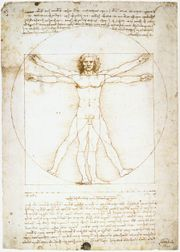
\includegraphics[width=4cm]{Vitruvian.png}
   \caption{Virtuvian Man}
   \label{Fig:vitruvian}
\end{figure}

The application must be able to handle data from average humans. It does not matter what the race or sex of the person is. The length of the person must be relatively average. This is to ensure that the proportions are correct.

\subsubsection{Head}
The human head is situated at the center of the human body if we are viewing a human from the front. The head is situated on top of the shoulders. If a person is standing in a relaxed upright position with their arms pointing downwards the head will be the highest position of the body.

\subsubsection{Elbows}
The elbows are the connection between the upper and lower arms. If a person is standing in a relaxed upright position with the arms pointing downwards the elbows will be situated roughly halfway between the hands and the shoulders. The upper arm connects the elbow with the shoulder and the lower arm connects the elbow to the hand.

\subsubsection{Hands}
As defined in the previous subsection a hand is connected to the elbow by the lower arm. It may be assumed for the purpose of this project that a person has two hands.

\subsection{Video Noise}
Most videos that are commercially available today have some form of data compression to decrease the size of the video data. There are two types of data compression. Lossless data compression is when data is compressed and the uncompressed data is exactly the same as the original. Unfortunately most video data compression algorithms use lossy quality compression. This is when the uncompressed data is not the exactly the same as the original, but looks the same to the human eye.

This leads to a problem called video noise. Video noise is different between videos and also each subsequent frame in a video. When a video has the same background for every frame in the video it is possible to eliminate most of the noise in the video. This is because most noise is only small fluctuations in the values of the RGB components.

To eliminate this noise a filter needs to be applied to the data. This filter needs a small value called a threshold to indicate how much fluctuation is allowed in the RGB components of every pixel between each frame. This value must not be too high because we must still be able to decide if there is a fluctuation in the data or if there were motion between the two frames. 

%
%Definisie: filter
%


The value of the threshold for the noise filter needs to be tested against different sets of video data. We can assume that after enough tests a value can be found that will hold for the general case. This value will not be influenced by the size of the video, because we concentrate on each pixel component between frames and not how the pixels behave relative to their neighbours.

It may be assumed that video noise will be present in all input files. This video noise will only be from the encoding of the data and not from big differences in frames. Furthermore we only need to compensate for minimal camera movement or vibration, because we already made the assumption that all video files are static or contain a minimal amount of deviation.

\subsection{Data Extraction}
The most important aspect of this project is extracting the correct data from the video files, while still having a system that is capable of processing the data without intervention from the user. For the tracking application this would imply being able to track the hands with high accuracy. For the cutting application it would mean cutting at the correct positions in the file. We are interested in the hand gestures and thus we must find a way to extract the movement of the hands from the video frames. If we are able to extract the hands in the first frame and follow the movements of the hands in the subsequent frames we will succeed in our goals.

For data extraction it is important that it is possible to detect the hands in each frame. If a hand can not be detected an estimate of its possible position must be made for the frames where it is missing.

A suitable method must be found to extract the data. In the next section we will look at possible methods of doing this. Before a method can be proposed we must know what constraints are to be placed on this method. Firstly when data extraction is performed we must only concentrate on areas that has previously contained or currently contains human body parts. We therefore have to assume a static background for each video.

To accurately determine what areas contain body parts we want the body parts to be distinct in each frame. Because this is a non-interactive system body parts will have to be determined from pixel values. For distinct areas a person whose skin tone does not have the same colour as the rest of the frame this would be ideal. Unfortunately we can not place this constraint on this project. We therefore assume that each frame may contain any permutation of possible pixel values.

The user must be able to vary the values needed to apply the extraction. This is to compensate for the possible situation that the default values do not provide correct results.

\subsection{Hand Movement Tracking}
The tracking of the movement of the hands must be applied on every frame. It is not necessary that the estimate of where the hands are situated in each frame is the same position on the hand. This means we only want an estimate of the general area where the hand may be situated. Overall only a small margin of error is allowed in the tracking of the hands. When an error occurs we must be able to compensate for the error and still provide correct tracking in the subsequent frames. This means the tracking error may give different hand positions than the input video, but must still provide tracking that is correct for a general case of the hand gesture associated to this video.


\subsection{Output Coordinates}
The output coordinates of the tracking of the hands can not be the same coordinates as the video coordinates. This is because different videos have different dimensions. The coordinates must be relative to the size of the head as well as the position of the center of the head.

\subsection{Video Cutting}
When a video needs to be cut into smaller parts, it can be assumed that the video contains parts where cutting may occur. A cut happens between two different hand gestures. An optimal choice would be when the character is standing still between the gestures. When determining if a cut must be made we rather want the situation where a possible cut is missed than a situation where we cut in the middle of a gesture.

\newpage
%
% PROTOTYPES AND DESIGN
%

\section{Prototypes and Design}

\subsection{Video Input Format}
As specified in the previous section, only MPEG-2 video files are considered as viable input files. Two possibilities were considered to load the video file into the application. The first was to interface with a video codec layer, which would allow us to handle other types of video codecs as well. Unfortunately this does not allow direct manipulation of the pixel components of each frame in a video because the video would have to be played through the Video4Linux \cite{v4l} API layer.

Therefore, a MPEG-2 decoder needs to be integrated into the application. I decided to modify an existing MPEG-2 library, which I obtained from The MPEG Software Simulation Group (MSSG) \cite{mpeg}. This allows me to directly access each video frame as it is being read. For the tracking application the whole video file is loaded into memory at once. This is done because a lot of operations need to be done on the data and by loading the data only once the amount of disk reads is kept to a minimum. The video frames are stored as a vector list in memory to allow a sequential read of each frame from the first frame as well as indexing to specific frames. At each frame the RGB values of each pixel, as well as the dimensions of the frame, is stored.

For the cutting application, which uses longer videos, the video file is not read into memory because each frame is only accessed once to determine if there is movement. This is done because uncompressed video data uses a lot of memory.

\subsection{Video Noise}
We know that each RGB component of a pixel is an 8-bit value. Thus the intensity of each component ranges from 0 to 255. Video noise from each frame is considered to be fluctuations in the intensities of each pixel if we follow the assumption from the formal description. Video noise can be detected by examining the differences between frames. According to \cite{colorclassifier} the best method to test for movement in videos is colour segmentation. Through testing I found that values that change less than 20\% of the maximum intensity can be considered to be video noise and all changes above this is movement in the video.

\subsection{Body Information Extraction}
Before movement of the hands can be tracked in a video, we must find the person standing in the video. We are trying to find the hands in each frame, thus we must find a way to easily detect body parts in each frame. The following subsections describe the order in which we obtain enough data to successfully track the hands later.

\subsubsection{Edge Detection}
Edge detection is the detection of movements between frames. This is called edge detection or colour segmentation \cite{colourclassifier} because the movements are picked up at the edges of areas where objects move over other objects.

In the case of human movement, this enables us to pick up areas that may have previously contained a human body part. We find these areas by applying a threshold value. If a value is over this threshold we can assume movement occurred. This threshold is all intensity values over the video noise boundary from the previous section. From \cite{movement} we have the following definition of image intensity \emph{I} between subsequent frames
\begin{displaymath}
I(x+u_x(x,y),y+u_x(x,y),t) = I(x,y,t+1)
\end{displaymath}

Movements between two frames are not enough to determine the outline of a human body. Therefore we need to find the mean and standard deviation of all the RGB components of each detected edge in the entire video. From mathematical statistics \cite{statsboek} we find that the most suitable method is the estimation of the mean $\mu$ and standard deviation $\sigma$, because the amount of pixels \emph{n} involved is not known before hand. It is calculated as follows
\begin{displaymath}
{X_{i,j}} =
\Bigg{\lbrace} \begin{array}{ccc}
Rgb_{i,j} & & when\;Rgb_{i,j} \geq motion\_threshold \\
0 & & when\;Rgb_{i,j} < motion\_threshold
\end{array} 
\end{displaymath}
\begin{displaymath}
n = number\; of\; pixels\; over\; motion\_threshold
\end{displaymath}
\begin{displaymath}
w = video\_width
\end{displaymath}
\begin{displaymath}
h = video\_height
\end{displaymath}
\begin{displaymath}
\mu = \frac{1}{n} \sum_{i=0}^{w-1}\sum_{j=0}^{h-1} X_{i,j}
\end{displaymath}
\begin{displaymath}
\sigma^2 = \frac{1}{n - 1} \sum_{i=0}^{w-1}\sum_{j=0}^{h-1} (X_{i,j} - \mu)^2
\end{displaymath}
\begin{displaymath}
\sigma = \sqrt{\sigma^2}
\end{displaymath}

If we now apply a simple test,
\begin{displaymath}
\mu - Edge\_threshold *\sigma < RGB(i,j)
\end{displaymath}
we are able to find the edges in every frame with high accuracy, as in Fig. \ref{Fig:edge}. If we examine the equation we can see that we look at the mean RGB value at each pixel and allow a small fraction, the edge threshold, of deviation from the mean.

\begin{figure}[htbp]
   \centering
   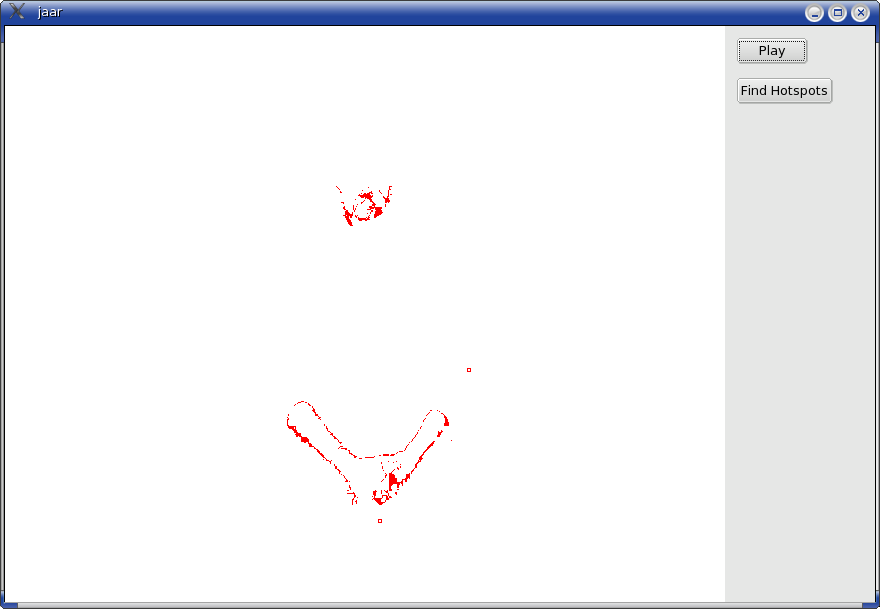
\includegraphics[width=10cm]{edge.png}
   \caption{Detected edges}
   \label{Fig:edge}
\end{figure}

\subsubsection{Body Part Isolation}
The edges do not give enough information about the human body parts to successfully track movement. We now need to determine from the edges in the first frame where the head, elbows and hands are. The first frame is inspected because all movement starts from there. Furthermore, it can be assumed that the video data used in this project will always have a first frame where the person is standing upright, with the elbows below the head and the hands below the elbows.

This assumption makes it possible to isolate certain body parts in the video. We want to isolate the head because in later frames it may happen that a hand passes over the face. If this happens we want an estimate of what area of the video the head is situated in. If we take our assumptions and the information from Section 3.3 into account, we can detect the head in the center of the upper half of the first frame. We must check the edges to find the correct position.

Once we have found the head we must find the elbows and hands. From the assumption that the person is standing in a relaxed upright position, we can find the center line of the body, thus allowing us to calculate the left and right hand sides of the body.

We know the elbows are initially situated above the hands and if we look at the highest edges on the left and right of the center line, we will find the relative positions of the two elbows.

The hands are isolated the same way as the elbows. The difference is that we now know that they are situated at the bottom of the frame. Again a search is conducted for the best fit for the left and right hands. Because we have defined a center line for the body, it does not matter if the hands are folded over each other because the relative positions will still be computed.
\subsubsection{Skin Tone Selection}
The skin tone is the last important detail we need. Together with the edges it will enable us to successfully find body detail in each frame. To compute the skin tone we need the mean and standard deviation of the RGB components of the lower arms. Using the information from the previous subsection, we are able to roughly determine a linear equation for each lower arm. By testing coordinates against these equations the mean and standard deviation of the lower arms can be computed.

\subsection{Hand Movement Tracking}

Detection of the hands is done seperately from each other on each frame. After careful consideration, three methods were developed to compute the tracking information of the hands.

\subsubsection{Linear Equation Model}
To find the hands in each frame, a linear equation needs to be formed for each arm from the previous frame. If a previous frame is not available the information gathered from the previous section must be used.

Once the equations have been created all possible areas that contain skin must be identified. This is done by applying the following test:

\begin{displaymath}
\mu - Skin\_threshold *\sigma < RGB(i,j)
\end{displaymath}

For each pixel identified as skin, it must be tested against an oriented bounding box \cite{obb} that is created from the equations derived previously for the arms. An oriented bounding box is an axis aligned bounding box \cite{aabb} that has been translated into new coordinates by applying axis translations. Fig. \ref{Fig:boxes} shows the difference between the two. In this case the oriented bounding box is a rectangular area that is projected on the equation of each arm. The pixels that fall in the bounds of the bounding box are then marked for use in the creation of new equations for the arms.

\begin{figure}[htbp]
   \centering
   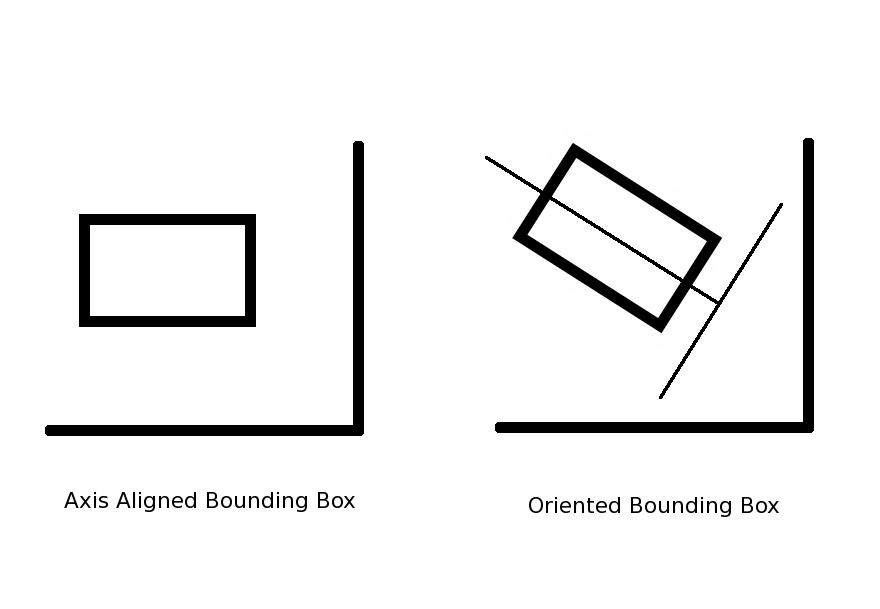
\includegraphics[width=10cm]{boxes.png}
   \caption{Types of bounding boxes}
   \label{Fig:boxes}
\end{figure}

As suggested \cite{whyleast} the method of least squares was chosen as the most suitable method. The method of maximum likelihood estimators, which according to \cite{statsboek} is an excellent estimator, is based upon this method. Once all the pixels have been checked, the linear least squares algorithm \cite{leastsquare} is used to compute a possible new equation for each arm. The following algorithm is performed on the marked pixel data.

\begin{displaymath}
a = \frac{\sum{y}  \sum{x^2} - \sum{x}\sum{xy}}{n\sum{x^2}-(\sum{x})^2}\\
\end{displaymath}
\begin{displaymath}
b = \frac{n\sum{xy}-\sum{x}\sum{y}}{n\sum{x^2}-(\sum{x})^2}\\
\end{displaymath}
\begin{displaymath}
y = a+bx
\end{displaymath}

This new equation is now used to find the possible positions of the elbows. Once this has been determined we can obtain an estimate of the position of the hands using the angle $\theta$ of the gradient \emph{m} of the equation and the length \emph{L} of the arm. This is done by using trigonometric functions \cite{trig} which is derived from Fig. \ref{Fig:triangle}.

\begin{displaymath}
\theta = cos^{-1}(m_{left})
\end{displaymath}
\begin{displaymath}
x_{left\_hand} = x_{left\_elbow} + L_{left\_arm} \times cos(\theta)\\
\end{displaymath}
\begin{displaymath}
y_{left\_hand} = y_{left\_elbow} + L_{left\_arm} \times sin(\theta)\\
\end{displaymath}
\begin{displaymath}
\theta = cos^{-1}(m_{right})
\end{displaymath}
\begin{displaymath}
x_{right\_hand} = x_{right\_elbow} - L_{right\_arm} \times cos(\theta)\\
\end{displaymath}
\begin{displaymath}
y_{right\_hand} = y_{right\_elbow} - L_{right\_arm} \times cos(\theta)\\
\end{displaymath}

\begin{figure}[htbp]
   \centering
   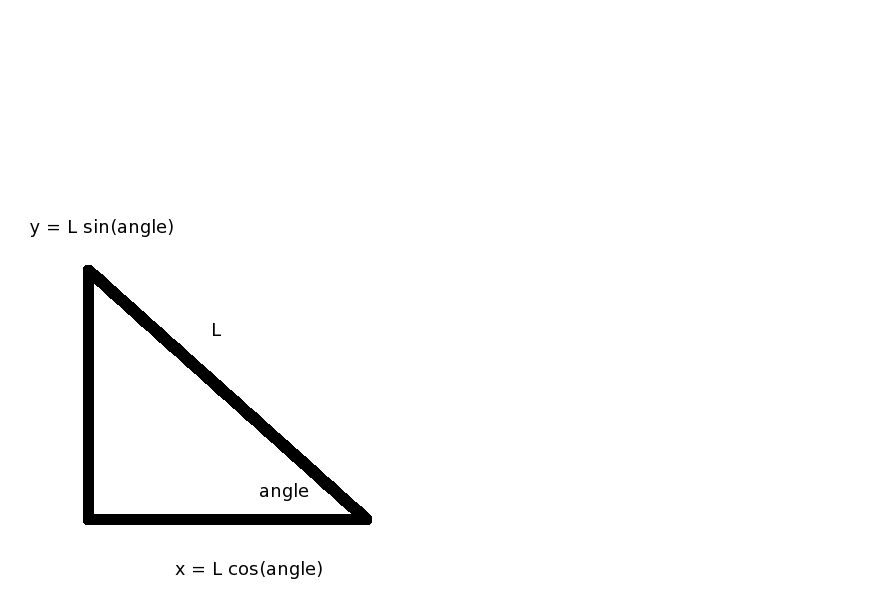
\includegraphics[width=10cm]{trig.png}
   \caption{General right triangles}
   \label{Fig:triangle}
\end{figure}

This, however, only provides us with a relative estimate of the position of the hands. This is because we are viewing the video in two dimensions, but the hands are moving in three dimensions. To integrate this problem into the algorithm, the Euclidean distance \cite{trig}, which is computed as
\begin{displaymath}
d(P_1,P_2)=\sqrt{ (x_2-x_1)^2 + (y_2-y_1)^2 + (z_2-z_1)^2}
\end{displaymath}
between two points, is used to find the nearest possible skin match to the estimate. If a new estimate could not be found the old estimate is used.

\subsubsection{Vector Motion Method}
The vector motion method is based upon first order kinematic equation models. This method was chosen \cite{aslgesture} to model the movement of single hand gestures in basic American Sign Language (ASL). Therefore it can be assumed that this is a tested method for modelling the behaviour of hand movement in sign language. It must be noted that basic ASL differs from SASL in one important aspect, namely that basic ASL is performed with one hand and SASL with two hands.

Tracking in this method is performed on the position of the hands alone. Each hand is assigned variables that correspond to its position and velocity. The velocity \emph{v} is computed as the displacement of the hand position between two subsequent frames and the estimate of new hand positions \emph{s}, as the integral taken over time and velocity \cite{physics}. This now allows us to define the following two equations for calculating the hand velocity and positions:

\begin{displaymath}
v(x,y,t) = \frac{\Delta{v}}{\Delta{t}}
\end{displaymath}
\begin{displaymath}
s(x,y,t+1) = s(x,y,t)+\int^{t+1}_t vdt = s(x,y,t) + v(x,y,t)( (t+1) - t)
\end{displaymath}

These two equations are then applied to each frame of the video to obtain estimates of the position of the hands. As in the previous method this only provides relative estimates of the position of the hands. Therefore the Euclidean distance is computed again to find the nearest skin match of the new hand position estimates.

As stated before SASL uses two hands and basic ASL one hand, this tends to lead to a problem with initial tracking because the hands may be initially positioned close to each other. To eliminate this problem the first ten frames are still tracked using the linear equation model. This allows the system to build up enough information about the hands as well as allowing the hands to move away from each other.
\subsubsection{Hybrid Method}

The hybrid method, which I developed from the previous two methods, is based upon the linear equation model and uses the same method for computing the position of the hands. The difference is the way in which the positions of the elbows are computed. Previously the elbows were determined as the widest position of the body. In the hybrid method the position of the elbows are estimated by using the vector motion model on the elbows. This method does not present satisfactory results and therefore it is not advised to use this method.

\subsection{Output Format}
The output format file contains information associated with the video followed by the two dimensional coordinates of each hand in each frame. The information put in the file is the name of the video file followed by the associated gesture and then the size of the video and the position of the person's chin.

The left hand coordinates, of the person, is put first followed by the right hand's coordinates. Every coordinate is relative to the position of the person's chin in the video. Below is an example of a possible output file for the gesture associated with the word \emph{apple}. These are not actual values.

\begin{verbatim}
#File Name
/mnt/removable/jaar projek/PartA_008.mpg
#Gesture
Apple
#Width Height Position_of_chin(x,y) 
720 576 364,205
#Left(x,y) Right(x,y) 
3,-261 0,-263
-3,-267 4,-268
0,-261 3,-268
-1,-260 3,-258
2,-246 -2,-254
-1,-245 5,-250
3,-224 4,-236
6,-208 0,-203
5,-185 -1,-155
27,-106 15,-101
22,-92 36,-61
11,-55 50,-46
-34,-50 66,-24
-51,-45 68,-11
-52,-40 65,-2
-49,-35 60,5
-50,-29 55,8
-50,-25 50,9
\end{verbatim}

\subsection{Video Cutting}
Video cutting is done by monitoring the edges, using the same technique specified in Section 4.3.1. The video is monitored for changes to the position of the hands. Specifically the area around the person's waist is monitored. This is done because we know that between gestures the hands must move past the waist. Once we find that the hands moved away from the waist and came back, and there was no movement for a second, we can consider a cut. One second corresponds to 25 frames on a standard 25 frames per second video. To actually perform a cut, movement must have occurred since the previous cut of the file. To cut the file, mpgcut \cite{mpgcut} was incorporated into the application. 


\subsection{User Interface}
I decided to implement a graphical user interface (GUI) for this project. This allows the viewing of the MPEG-2 videos. GTK+ \cite{gtk} and Qt \cite{qt} was considered as APIs to implement the interface in. The project must work in a Linux environment and these are the most popular GUI APIs available in Linux. I decided to use the Qt API as this is the native API of the KDE window manager, in which this application is being developed. It must be noted that both APIs have a Windows API as well.

The GUI does not have a preset size and rather adapts to the size of the video that is currently being processed. Three buttons, three sliders and a dropdown list are present on the interface (see Fig. \ref{Fig:gui}). The buttons allow the playing, pausing and tracking of the video, the opening of a Mpeg file, and the saving of tracking information respectively. The first two sliders allow changing the edge and skin threshold values from the default values. If an incorrect estimate of the hands were made this will allow the user to try different configurations and hopefully obtain correct results. The third slider shows what position in the video is currently being processed. The dropdown list enables the user to select which method must be used to calculate the tracking of the hands. It must be noted that the video can be paused while being processed and the user can then select another method. 

\begin{figure}[htbp]
   \centering
   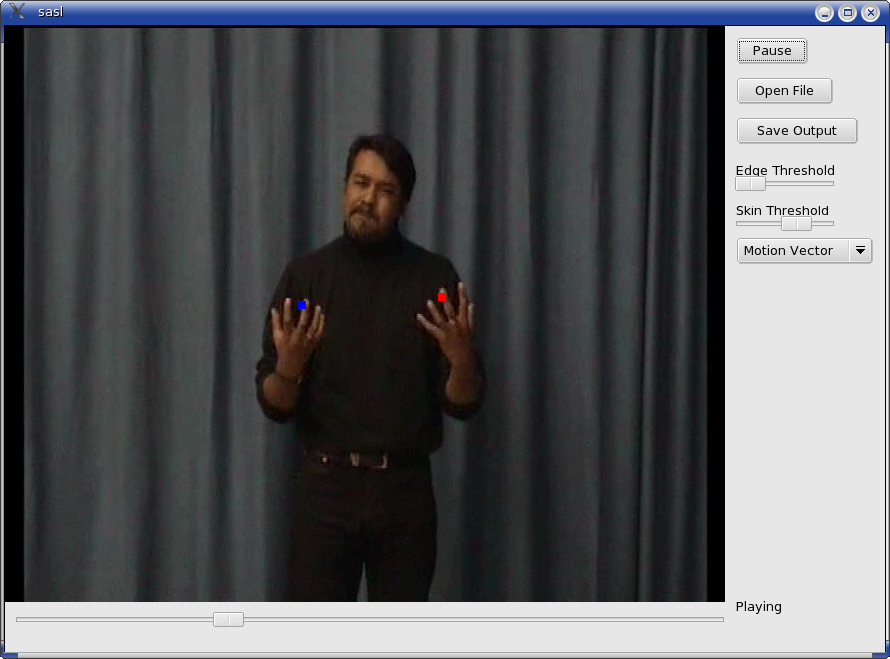
\includegraphics[width=10cm]{gui.png}
   \caption{Graphical User Interface}
   \label{Fig:gui}
\end{figure}

\newpage
%
% TESTING
%
\section{Testing}
Testing was conducted on a set of video files. This was to assess the quality of the methods which are used to track hand movement in each video file and to find possible situations that may hinder this tracking.

For these tests the application was executed with the default parameter values. This means the application was tested with the threshold slider values at the initial positions. The test set consisted of a set of 190 video files and another set of 105 files.

From these tests I could conclude that my method works satisfactorily, but still fails in some cases. After inspection I found that there are two distinct cases which produce incorrect results. The first case occurs when the person's hands move to fast, which leads to some frames in the video where the pixels are distorted too much and a hand can not be identified (see Fig. \ref{Fig:fast}). These errors are not because of a deficiency in the application but rather because of inconsistent video frame data. In these cases the user is advised to use the motion vector method.

The second case occurs when a person's hand moves past $90^o$ (see Fig. \ref{Fig:perp}). This leads to an incorrect estimation of the position of the elbow, which in turn leads to an incorrect estimation of the position of the hand. This error can be avoided by applying the vector motion method in the right manner. In general all video files that did not contain one of the previous cases the results were correct.

\begin{figure}[p]
   \centering
   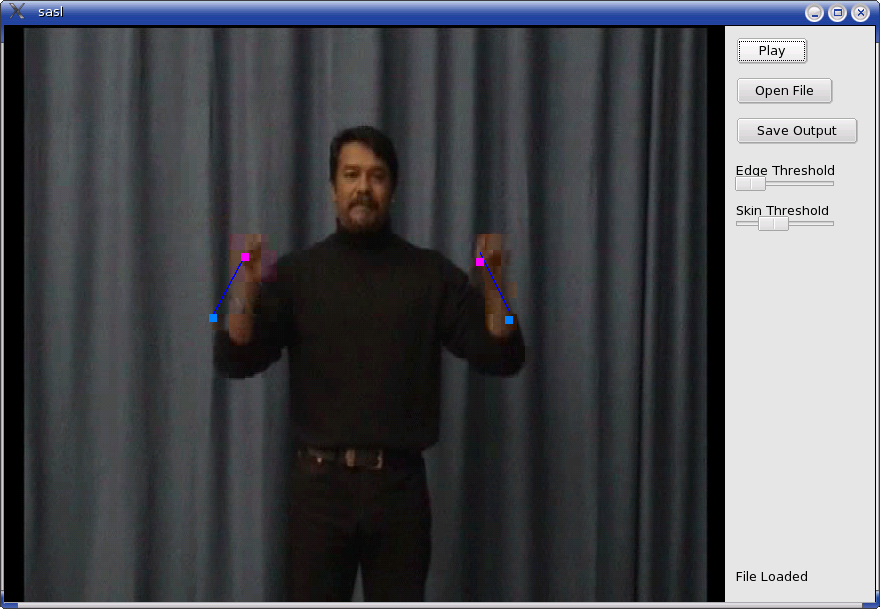
\includegraphics[width=10cm]{fast.png}
   \caption{Error Case 1}
   \label{Fig:fast}
\end{figure}

\begin{figure}[p]
   \centering
   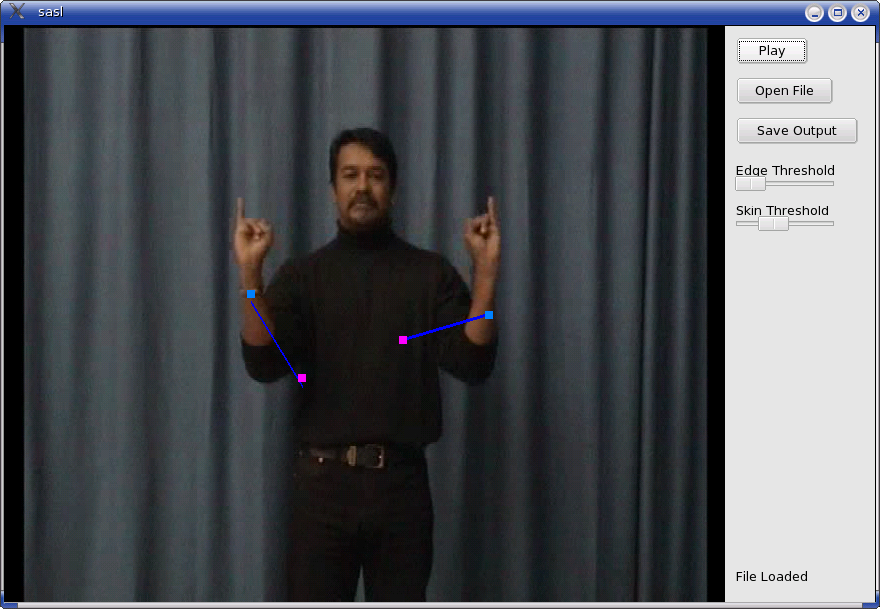
\includegraphics[width=10cm]{perp.png}
   \caption{Error Case 2}
   \label{Fig:perp}
\end{figure}

\newpage
%
% FUTURE WORK
%
\section{Future Work}
\subsection{Hand Movement Tracking}
I feel that possibly the most important aspect of any program, that is developed today, is how portable the application is. My tracking application currently has only been tested in a Linux environment and if possible this should be done in a Windows environment in the future. Because the Qt API, which is compatible with both environments, was used and no other external libraries was used, it should not be difficult.

Currently, when a video is being played and tracked in the program, the playing is done sequentially as expected, but the user is not allowed to move around to any position in the video and start playing the video from there. If this is to be implemented, another feature could be added. In the situation where an incorrect decision could have been made about the position of the hand, the user could then be allowed to change this decision 

One last feature that can be implemented is to possibly process other video formats.

\subsection{Video Cutting}
The video cutting application is a small stand alone console application. To change this, the cutting application could possibly be integrated into the tracking application. This would allow one application that does all the work, which would increase the productivity of the whole data collection process from start to end.

As with the tracking application, the cutting application can also be modified to allow the cutting of different video formats.
\newpage
%
% REFERENCES
%
\begin{thebibliography}{20}

\bibitem{aabb} Axis Aligned Bounding Box,
\emph{Bounding Volume - Wikipedia, the free encyclopedia},	
[Online], Available from \emph{http://en.wikipedia.org/wiki/Bounding\_volume}

\bibitem{whyleast} Charles Stewart,
\emph{Robust Parameter Estimation in Computer Vision},	
1999.

\bibitem{movement} Cristoph Bregler and Jitendra Malik,
\emph{Tracking People with Twists and Exponential Maps},	
1998.

\bibitem{statsboek} Dennis Wackerley, William Mendenhall and Richard Scheaffer,
\emph{Mathemathical Statistics with Applications},
Duxbury, 6th Edition, 2002.

\bibitem{leastsquare} Howard Anton and Chris Rorres,
\emph{Elementary Linear Algebra},	
John Wiley \& Sons, 8th Edition, 2000.

\bibitem{physics} Hugh Young and Roger Freedman,
\emph{University Physics},	
Sears and Zemansky's, 10th Edition, 2000.

\bibitem{trig} James Stewart,
\emph{Calculus: Fourth Edition},
Brooks/Cole Publishing Company, 4th Edition, 1999.

\bibitem{gtk} GTK+,
\emph{GTK+ - The GIMP Toolkit},	
[Online], Available from \emph{http://www.gtk.org/}.

\bibitem{aslgesture} Konstantinos Derpanis, Richard Wildes and John Tsotsos,
\emph{Hand Gesture Recognition within a Linguistics-Based Framework}.

\bibitem{mpeg} The MPEG Software Simulation Group,
\emph{MPEG.ORG - MPEG Software Simulation Group (MSSG)},	
[Online], Available from \emph{http://www.mpeg.org/MPEG/MSSG/}

\bibitem{mpgcut} mpgcut,
\emph{mpgcut a command line MPEG file cutter},	
[Online], Available from \emph{http://mpgcut.sourceforge.net/}

\bibitem{obb} Oriented Bounding Box,
\emph{flipcode - 2D OBB Intersection},	
[Online], Available from \emph{http://www.flipcode.com/cgi-bin/msg.cgi?showThread=COTD-2DOBBIntersection\&forum=cotd\&id=-1}

\bibitem{qt} Qt,
\emph{Qt - Trolltech},	
[Online], Available from \emph{http://www.trolltech.com/products/qt}.

\bibitem{colorclassifier} Richard Schumeyer and Kenneth Barner,
\emph{A Color-Based Classifier for Region Identification in Video}.

\bibitem{v4l} Video4Linux,
\emph{Main Page - V4LWiki},	
[Online], Available from \emph{http://www.linuxtv.org/v4lwiki/index.php/Main\_Page}

\bibitem{wiki} Wikipedia, the free encyclopedia,
\emph{Body Proportions - Wikipedia, the free encyclopedia},	
[Online], Available from \emph{http://en.wikipedia.org/wiki/Body\_proportions.htm}

\end{thebibliography}
\end{document}


